\documentclass[12pt,a4paper]{article}
\usepackage[utf8]{inputenc}
%\usepackage[german]{babel}
\usepackage{amsmath}
\usepackage{amsfonts}
\usepackage{amssymb}
\usepackage{amsthm}
\usepackage{graphicx}
\usepackage{xcolor}
\usepackage[backend=bibtex,bibencoding=ascii,style=numeric,sorting=none]{biblatex}
\usepackage{slashed}
\usepackage{xcolor}
\addbibresource{source.bib}


\author{Julian Köberle}
\title{Notes on fermions in curved space}
\begin{document}
	\maketitle
	
	\newcommand{\np}{\slashed{\partial}}
	\newcommand{\nG}{\slashed{\Gamma}}
	\newcommand{\nn}{\slashed{\nabla}}
	\newcommand{\overbar}[1]{\mkern 1.5mu\overline{\mkern-1.5mu#1\mkern-1.5mu}\mkern 1.5mu}\textbf{}
	
	
	\newcommand{\tensor}[3]{{#1}^{#2}_{#3}}
	
	
	\begin{abstract}
		These are notes on my work studying the behavior of fermions in curved space. These notes may contain spelling errors, grammatical errors or stylistic inaccuracies and are therefore not intended for distribution to third parties.
		
	\end{abstract}
	
	\tableofcontents 
	
	
	\section{$\psi(x)$ in Minkowski space}
	The Dirac equation (DE) in flat Minkowski space reads as follows;
	\begin{equation}
		\label{diracEq}
		\left( i \np -m \right) \psi(x) = 0 
	\end{equation}

	where $\np = \gamma^\mu \partial_\mu$,
	
	One approach to solving the equation is by sepereting $\psi$ into an spinor and phase part:
	$$
	\psi(x) = u(\vec{p}) e^{i p^\mu x_\mu}
	$$
	Inserting the above expression one gets a usual matrix eigenvalue problem, it's quit handy to boost the system into a rest frame where $p^\mu = (m, \vec{0})$. This transformation reduces the DE quite dramatically such that one gets,
	
	$$
	(\gamma^0 - \mathbf{1} )u(m) = 0
	$$
	This equation has the following solutions;
	
	$$
	u^{(1)}\left({\vec {0}}\right)={\begin{bmatrix}1\\0\\0\\0\end{bmatrix}}\qquad u^{(2)}\left({\vec {0}}\right)={\begin{bmatrix}0\\1\\0\\0\end{bmatrix}}\qquad v^{(1)}\left({\vec {0}}\right)={\begin{bmatrix}0\\0\\1\\0\end{bmatrix}}\qquad v^{(2)}\left({\vec {0}}\right)={\begin{bmatrix}0\\0\\0\\1\end{bmatrix}}
	$$
	To get $u(p)$ in a none rest frame, one needs to boost $u(m)$ back to the moving system. 
	
	For a ortochronous propper lorentz transformation
	$$ 
	x \rightarrow x' = \Lambda x
	$$
	$$\psi(x) \rightarrow \psi'(x') = \Lambda_{1/2} \psi(x) \leftarrow \text{spinor-transformation-rule}$$
	
	follows
	$$
	\Lambda_{1/2}^{-1} \gamma^\mu \Lambda_{1/2} = \Lambda^\mu\,_{ \nu} \gamma^\nu 
	$$
	\footnote{Group theoretical proof outstanding}
	
	\begin{proof}
		The DE needs to hold for every reference frame, one makes the ansatz,
		$$\left( i \np' -m \right) \psi '(x') = 0$$ 
		with
		$$\partial'_\mu = {\Lambda^{-1}}^{\nu}\,_{\mu}  \partial_\nu $$
		$$\rightarrow \np' = \gamma^\mu {\Lambda^{-1}}^{\nu}\,_{\mu}  \partial_\nu$$
		follows
		$$\left( i \gamma^\mu {\Lambda^{-1}}^{\nu}\,_{\mu}  \partial_\nu -m \right) \Lambda_{1/2} \psi(x) = 0$$ 
		$$ \Lambda_{1/2}  \Lambda_{1/2}^{-1}\left( i \gamma^\mu {\Lambda^{-1}}^{\nu}\,_{\mu}  \partial_\nu -m \right) \Lambda_{1/2} \psi(x) = 0$$ 
		$$ \Lambda_{1/2}  i \Lambda_{1/2}^{-1} \gamma^\mu {\Lambda^{-1}}_{\ \mu}^{\nu}  \partial_\nu \left(\Lambda_{1/2} \psi(x)\right) -m   \Lambda_{1/2} \psi(x)= 0$$ 
		$$ \Lambda_{1/2} \left( i \Lambda_{1/2}^{-1} \gamma^\mu {\Lambda^{-1}}^{\nu}\,_{\mu}  \Lambda_{1/2} \partial_\nu -m \right) \psi(x) = 0$$ 
		because
		$$\left( i \np -m \right) \psi(x) = 0$$
		follows
		$$\Lambda_{1/2}^{-1} \gamma^\mu {\Lambda^{-1}}^{\nu}\,_{\mu}  \Lambda_{1/2} = \gamma^\nu$$
		$$\Lambda_{1/2}^{-1} \gamma^\mu {\Lambda^{-1}}^{\nu}\,_{\mu}   = \gamma^\nu \Lambda_{1/2}^{-1}$$
		$$\Lambda_{1/2}^{-1} \gamma^\mu \delta^\alpha_\mu   = \gamma^\nu \Lambda_{1/2}^{-1}\Lambda^\alpha\,_{\nu}$$
		$$\Lambda_{1/2}^{-1} \gamma^\alpha \Lambda_{1/2} = \gamma^\nu \Lambda^\alpha\,_{\nu}=  \Lambda^\alpha\,_{\nu} \gamma^\nu $$
	\end{proof}
	
	\section{Dirac equation in curved space}
	Equation (\ref{diracEq}) is only well-defined in flat space, because $\partial_\mu \Psi(x)$ does not transform under a general coordinate transformation like a spinor. Further the Dirac-algebra needs to be generalized to the generic the metric $g_{\mu \nu}$ which leads to the Clifford-algebra. Since GR is defined on a manifold $\mathcal{M}$, it is possible to choose a coordinate system, that is locally flat with Lorentzian signature. In order to manifest these circumstances in a mathematical formalism, the \textit{vierbein} or \textit{tetraed} formalism is suitable, which is worth studying more closely.
	
	\begin{equation}
		\label{tetraed}
		g_{\mu \nu}(x)  e_a\,^{\mu}(x) e_b\,^{\nu}(x) = \eta_{a b}
	\end{equation}
	Equation (\ref{tetraed}) is the \underline{local} coordinate transformation connecting the metric $g_{\mu \nu}(x) $ defined in curved space-time and  Minkowski metric $\eta_{ab}$. Here $e_a\,^\mu(x)$ are the so-called tetraeds. To distinguish flat from general coordinates, Greek indices $\mu,\nu,\ldots$ are used for curved space and
	Latin indices $a,b,c,\ldots$ are therefore used for the local flat space. In order not to overload the notation, $x$ dependencies are suppressed, and we write $g_{\mu\nu} = g_{\mu\nu}(x)$ and $e_a\,^{ \mu } = e_a\,^{ \mu}(x)$.
	A relation for the inverse metric can be defined analogously,
	
	
	\begin{equation}
		\label{tetraed}
		g^{\mu \nu}  \tilde{e}_\mu\,^{a} \tilde{e}_\nu\,^{b} = \eta^{a b}
	\end{equation}
	 $e$ and $\tilde{e}$ are generally different objects, but since the index position of the Greek or Latin index clearly defines whether it is either $e$ or $\tilde{e}$ the " $\tilde{}$ " is omitted, but care must be taken, when expressions are explicitly written in components; since e.g. $e^2_2 \neq \tilde{e}^2_2$.
	Further, because of
	$$g^{\mu\nu}g_{\nu\alpha}=\delta^\mu_\alpha$$
	follows: 
	$$
	e_a\,^{\mu}e_\mu\,^{b} = \delta_a^b \ , \ \ e_a\,^{\nu} e_\mu\,^{a} = \delta_\mu^\nu
	$$
	A general tensor $T^{\mu_1 \mu_2 \ldots \mu_l}\,_{\nu_1 \nu_2 \ldots \nu_p}$ can be written in flat coordinates as the following,
	
	

	\begin{equation}
		T^{a_1 a_2 \ldots a_l}\,_{b_1 b_2 \ldots b_p} =  e_{\mu_1}\,^{ a_1} e_{\mu_2}\,^{a_2} \ldots e_{\mu_l}\,^{a_l} e_{b_1}\,^{ \nu_1} e_{b_2}\,^{\nu_2} \ldots e_{b_p}\,^{\nu_p} T^{\mu_1 \mu_2 \ldots \mu_l}\,_{ \nu_1 \nu_2 \ldots \nu_p}
	\end{equation}
	and vice versa.
	
	\subsection{Covariant derivative}
	A derivative acting on vectors, or more generally on tensors, is a mathematical "tool" that measures the change in spacetime. Unfortunately, the expression $\partial_\mu V^\nu$ has in general no tensorial behavior. If a general coordinate transformation $\partial x^\alpha/ \partial x'^\nu$ acts on $\partial_\mu V^\nu$, terms of the second derivative arise which destroy the tensorial behaviour.
	 
	
	Furthermore, a comparison of tensors that are spatially separated live in different tangential spaces, therefore a naive comparison is not properly defined. In order to compare two tensors from two distinct tangential spaces, one tensor must be shifted auto parallel from one space $T_P\mathcal{M}$ to the other one $T_Q\mathcal{M}$.
	
	
	It makes sense to define a covariant derivative $\nabla_\textbf{v}$, where $\textbf{v} \in T_P\mathcal{M}$. If $\textbf{u} : \mathcal{M} \mapsto T\mathcal{M}$ is a vector field defined on the manifold, then $\nabla_\textbf{v}\textbf{u} |_P$ is the change of $\textbf{u}$ towards $\textbf{v}$ at point $P$, this expression can easily be rewritten in index notation by using
	$\textbf{u} = u^\alpha(x) \partial_\alpha$ and $\textbf{v} = v^\beta(x) \partial_\beta$. For the effect on basis vectors it makes sense to define a connection in the following way $\nabla_{(\partial_\beta)}(\partial_\alpha) = \Gamma^\mu\,_{\alpha \beta} \partial_\mu$ (at this point, no clear definition on $\Gamma$ has been made, only the fact, it cancels the terms of second order derivative, which would arise by transforming $\partial_\mu V^\nu$ but it's not a unique definition, to make the covariant derivative properly tensorial). Inserting of $\textbf{u}$ and $\textbf{v} $ into $\nabla_\textbf{v}\textbf{u} |_P$ gives,
	
	\begin{multline}
		\label{kovariant}
		\nabla_{v^\beta \partial_\beta}(u^\alpha(x) \partial_\alpha) = v^\beta \nabla_{(\partial_\beta)} (u^\alpha(x)\partial_\alpha ) = v^\beta \left(\nabla_{(\partial_\beta)} (u^\alpha(x)) \partial_\alpha +  u^\alpha(x) \nabla_{(\partial_\beta)} \partial_\alpha \right)) \\ = v^\beta \left(\partial_\beta u^\alpha(x)  \partial_\alpha +  u^\alpha(x) \Gamma^\mu\,_{\alpha \beta} \partial_\mu\right)  \\ = v^\beta \left(\partial_\beta u^\alpha(x)   +  u^\mu(x) \Gamma^\alpha\,_{\mu \beta}\right) \partial_\alpha 
	\end{multline}
	The second term is obtained, by using linearity of $T_P\mathcal{M}$, the second by the product rule of the derivation. The third by substituting $\Gamma$ and using the fact, that a covariant derivation of scalars reduces to conventional derivations. The last expression is obtained by index renaming. This expression is valid for all $v^\beta$, therefore it follows for the covariant derivation in index notation,
	
	\begin{equation}
		\label{covariant}
		\nabla_\beta u^\alpha = \partial_\beta u^\alpha  +   \Gamma^\alpha\,_{\mu \beta} u^\mu
	\end{equation}
	
	because of $\nabla_\beta \left(u^\alpha u_\alpha\right) = \partial_\beta \left(u^\alpha u_\alpha \right)$ 
	follows
	
	$$\nabla_\beta u_\alpha = \partial_\beta u^\alpha  -   \Gamma^\mu\,_{\alpha \beta} u_\mu$$.
	
	By doing this procedure for $\nabla_\beta u^\mu u^\nu \ldots$ one gets the behaviour  of a general tensor  $T^{\mu_1 \mu_2 \ldots \mu_l}\,_{\nu_1 \nu_2 \ldots \nu_p}$ acting with a covariant derivative. Additionally, it makes a lot of sense to define the connection torsion free which means,
	$$
	\Gamma^\rho\,_{\alpha \beta} = \Gamma^\rho\,_{\beta \alpha}.
	$$
	This is similar by demanding metric-compatibility, which in other words means the covariant derivative acting on $g^{\mu \nu}$ gets annihilated, $\nabla_\alpha g_{\mu \nu} = 0$. So the connections reads,
	
	
	\begin{equation}
		\label{christoffelconnection}
		\Gamma^{\sigma }\, _{{\mu }{\nu }}={\frac {1}{2}}g^{{\sigma }{\kappa }}\left({\frac {\partial g_{{\nu }{\kappa }}}{\partial x^{\mu }}}+{\frac {\partial g_{{\mu }{\kappa }}}{\partial x^{\nu }}}-{\frac {\partial g_{{\mu }{\nu }}}{\partial x^{\kappa }}}\right),
	\end{equation}
	Which is the well known Christoffel-symbol.
	
	It is now interesting to know how the covariant derivatives acts on $u^a$. One makes the the following approach,
	
	\begin{equation}
		\label{dua}
		\nabla_\beta u^a = \partial_\beta u^a + \omega_{\beta b}\,^{a}u^b
	\end{equation}
	using the fact that the above expression transforms like a $T_{\beta}\,^{a}$ tensor, it is useful to rewrite it in the basis of general coordinates.  
	$$
	\nabla_\beta u^a = e_\alpha\,^a \nabla_\beta u^\alpha 
	$$
	expanding $\nabla_\beta$ usign eq. (\ref{covariant}) and eq. (\ref{dua}),
	$$
	 \partial_\beta u^a + \omega_{\beta b}\,^{a}u^b = e_\alpha\,^a \left(  \partial_\beta u^\alpha  +   \Gamma^\alpha\,_{\mu \beta} u^\mu \right)
	$$
	$$
	 = \partial_\beta(\underbrace{u^\alpha e_\alpha\,^a}_{u^a}) - u^\alpha \partial_\beta (e_\alpha\,^a) +  e_\alpha\,^a   \Gamma^\alpha\,_{\mu \beta} u^\mu 
	$$
	$$
 \Rightarrow - u^b e_b\,^{\alpha} \partial_\beta (e_\alpha\,^a) +  e_\alpha\,^a   \Gamma^\alpha\,_{\mu \beta} u^b e_b\,^{\mu}  =  \omega_{\beta b}\,^{a}u^b
	$$
	for all $u^b$ follows
	\begin{equation}
		 \omega_{\beta b}\,^{a} = \Gamma^\alpha\,_{\mu \beta} e_b\,^{\mu} e_\alpha\,^a    - e_b\,^{\alpha} \partial_\beta (e_\alpha\,^a) 
	\end{equation}
	renaming indices,
	\begin{equation}
		\label{omega}
		\omega_{\mu a b} = \eta_{b c}\Gamma^\alpha\,_{\nu \mu} e_a\,^{\nu} e_\alpha\,^c    - \eta_{b c} e_a\,^{\alpha} \partial_\mu (e_\alpha\,^c) 
	\end{equation}
	In contrast to $\Gamma^\alpha\,_{\mu \beta}$, $\omega_{\mu a b}$ transforms like a 2-form in $a,b$.
	
	\begin{proof}
		To show $\omega_{\mu a b}$ is antisymmetric in $a$ and $b$ it is convenient to contract this quantity with something symmetric like the Minkowski metric $\eta^{ab}$. 
		$$\omega_{\mu a b}\eta^{ab} \stackrel{?}{=} 0$$
		using eq. (\ref{omega}),
		$$\omega_{\mu a b}\eta^{ab} = \Gamma^\alpha\,_{\nu \mu} e_a\,^{\nu} e_\alpha\,^c \underbrace{\eta_{b c} \ \eta^{ab}}_{\delta_c^a}    -  e_a\,^{\alpha} \partial_\mu (e_\alpha\,^c)  \underbrace{\eta_{b c} \ \eta^{ab}}_{\delta_c^a}     $$
		$$ = \Gamma^\alpha\,_{\nu \mu} \underbrace{e_a\,^{\nu} e_\alpha\,^a}_{\delta_\alpha^\nu} -  e_a\,^{\alpha} \partial_\mu (e_\alpha\,^a)$$
		$$ = \Gamma^\nu\,_{\nu \mu} - e_a\,^{\alpha} \partial_\mu (e_\alpha\,^a)$$
		
		using the definition of the Christoffel symbols one gets,
		$$\Gamma^\nu\,_{\nu \mu} = \frac{1}{2}\left(g^{\nu \kappa}\partial_\mu g_{\nu \kappa}\right)$$
		inserting $ g_{\nu \kappa} = e_{\nu}\,^a e_{\kappa}\,^b \eta_{ab}$ and $ g^{\nu \kappa} = e_{a}\,^\nu e_{b}\,^\kappa \eta^{ab}$, gives $$\Gamma^\nu\,_{\nu \mu} =  e_a\,^{\alpha} \partial_\mu (e_\alpha\,^a)$$
		and therefore $\omega_{\mu a b}$ is antisymmetric in $a$ and $b$
		
		It is easy to see that $\omega_{\mu a b}$ transforms like a Lorentz tensor in $a$ and $b$ since a Lorentz transformation $\Lambda$ is not depended on $x$. 
		
		This concludes the statement $\omega_{\mu a b}$ transforms like 2-form in $a$ and $b$
		
	\end{proof}
	
	Finally, the covariant derivative on a spinor $\Psi(x)$ is as follows,
	
	\begin{equation}
		\label{DPsi}
		\nabla_\beta \Psi = \partial_\beta \Psi - \frac{1}{2} \omega_\mu^{\ a b }\Gamma_{(j)}(M_{a b})\Psi
	\end{equation}
	where $\Gamma_{(j)}$ is the spin-$j$ representation of the Lorentz algebra $\mathfrak{su}(1,3)$
	with $M_{a b} \in \mathfrak{su}(1,3)$ satisfying commutator relations,
	
	$$
	[M^{a b },M^{c d }]=M^{a d }\eta ^{b c }-M^{b d }\eta ^{a c }+M^{b c }\eta ^{a d }-M^{a c }\eta ^{b d }
	$$
	
	if $\Psi$ would have spin-1 it would transform as a vector $v^a$ and the corresponding representation would be:
	
	$$
	\Gamma_{(1)}(M^{a b }) = (M^{a b })_{c d }=\delta ^{a }{}_{c }\delta ^{b }{}_{d }-\delta ^{b }{}_{c }\delta ^{a }{}_{d },
	$$
	by pluggin in into eq. (\ref{DPsi}) one would get (\ref{dua}).
	
	But $\Psi$ is a spinor and has obviously spin-1/2 and therefore, the corresponding Lorentz representation is defined as follows,
	
	$$
	\Gamma_{(1/2)}(M^{a b }) = \frac{1}{4}[\gamma^a, \gamma^b].
	$$
	
	It is worth introducing the so called spinor-connection which reads,
	
	$$
	\Gamma_\mu = -\frac{1}{8} \omega_{\mu a b}[\gamma^a, \gamma^b]
	$$

	which this definition the dirac equation in curved space finally reads,
	
	
	\begin{equation}
		\label{dirac_in_curved}
	\left(i\gamma^a \left( \partial_\alpha + \Gamma_\alpha \right)-m\right)\Psi = (i\nn - m)\Psi = 0
	\end{equation}
	\section{Curvature Tensor}
	So far, no metamathematical treatment what curvature actually means wasn't described yet.  We know by parallel-transporting a vector on a curved surface (imagine a shepere) it will show into a different direction when one would have chosen a different path. The difference between these two vectors parallel-transported over those paths, is what we call curvature. By taking the paths infinitesimal one gets the Riemann curvature tensor $R^\rho\,_{\alpha \beta  \gamma }$ defined the following,
	
	$$
	[\nabla_\mu, \nabla_\nu]v^\rho =  R^\rho\,_{\mu \nu \gamma } v^\gamma
	$$
	or,
	
	$$
	[\nabla_\mu, \nabla_\nu]v^a =  R^a\,_{\mu \nu b } v^b.
	$$
	
	Because $R^\rho\,_{\mu \nu \gamma }$ and $R^a\,_{\mu \nu b }$ are both tensors, it is possible to transform them into each other with,
	
	$$
	R^\rho\,_{\mu \nu \gamma } = e_a\,^\rho e_\gamma\,^b R^a\,_{\mu \nu b }
	$$
	
	and finally acting on a spinor one gets,
	$$
	[\nabla_\mu, \nabla_\nu]\psi = \frac{i}{4} R_{\mu \nu \alpha \beta} \sigma^{\alpha \beta} \psi.
	$$
	
	
	
	\section{Solution of dirac equation to $\mathcal{O} (\hbar^2)$}
	doing a WKB expanions,which means expanding $\psi$ in powers of $\hbar$ one writes,
	
	\begin{equation}
		\psi(x) = \exp(i S[x]/\hbar) \sum_{n=0}^{\infty}(-i\hbar)^n \psi_n(x)
	\end{equation}
	inserting into eq.(\ref{dirac_in_curved})
	follows,
	
	\begin{equation}
		\left(\gamma^\mu \partial_\mu S[x] + m \right)
	\end{equation}
	
	
	\begin{equation}
		\label{solution_to_diraceq}
		\psi(x) = \psi_0 \exp\left(\frac{i}{\hbar}\int dx^\mu p_\mu\right)
	\end{equation}
	\section{Corrections to 4-velocity and 4-acceleration}
	$$
	\ldots
	$$
	\begin{equation}
		\label{correction_to_v}
		v_\alpha = u_\alpha + \frac{\hbar}{mi}\overbar{\psi}_0 \Gamma_\alpha \psi_0 +\mathcal{O} (\hbar^2)
	\end{equation}
	$\ldots$
	\begin{equation}
		\label{correction_to_a}
		a_\alpha = v^\beta \nabla_\beta v_\alpha =  -\frac{\hbar}{4m} R_{\alpha \beta \gamma \delta}u^\beta \sigma^{\gamma \delta}
	\end{equation}
	
	
	
	\section{Effect by gravitational waves}
	By linearizing the Einstein Equation and neglecting matter sources one finds,
	
	$$
	g_{\mu \nu } = \eta_{\mu \nu } + h_{\mu \nu }e^{i k_\alpha x^\alpha} + \mathcal{O}(|h|^2)
	$$
	inserting this into the definition of the Christoffel-connection (\ref{christoffelconnection}) one finds,
	
	$$
	\Gamma^{\mu}\,_{\nu \alpha} = i\frac{1}{2}\eta^{\mu \beta}  \left(-h_{\nu \alpha} k_{\beta}+h_{\nu \beta} k_{\alpha}+h_{\beta \alpha} k_{\nu}\right)  \exp\left(i k_{\lambda} x^{\lambda}\right) +  \mathcal{O}(|h|^2)
	$$
	
	
	$$
	R^{\rho}\,_{\sigma \mu \nu} = \partial_\mu \Gamma^{\rho}\,_{\nu \sigma} - \partial_\nu \Gamma^{\rho}\,_{\mu \sigma} + \mathcal{O}(|h|^2)
	$$
	
	$$
	R^{\rho}\,_{\sigma \mu \nu} = i k_\mu \Gamma^{\rho}\,_{\nu \sigma} -  i k_\nu \Gamma^{\rho}\,_{\mu \sigma} + \mathcal{O}(|h|^2)
	$$
	
	$$
	R^{\rho}\,_{\sigma \mu \nu} = \eta^{\rho \beta}\left(k_\mu \left(k_\beta h_{\nu \sigma} - h_{\nu \beta}  k_\sigma \right) - k_\nu \left( k_\beta h_{\mu \sigma} - h_{\mu \beta}  k_\sigma\right) \right) \exp\left(i k_{\lambda} x^{\lambda}\right)  + \mathcal{O}(|h|^2)
	$$
	
	The geodesic equation is as follows,
	$$
	\frac{du^\alpha}{d \tau} = \Gamma^{\alpha}\,_{\mu \nu}u^\mu u^\nu
	$$
	$$%
	\Rightarrow
	\frac{du^\alpha}{d \tau} = 0
	\Rightarrow u^\alpha = const
	$$
	because otherwise the contraction of $R^{\rho}\,_{\sigma \mu \nu}u^\sigma$ would be of order $|h|^2$.
	
	$$
	R^{\rho}\,_{\sigma \mu \nu}u^\sigma = \left[\eta^{\rho \beta}\left(k_\mu \left(k_\beta h_{\nu \sigma} - h_{\nu \beta}  k_\sigma \right) - k_\nu \left( k_\beta h_{\mu \sigma} - h_{\mu \beta}  k_\sigma\right) \right) \exp\left(i k_{\lambda} x^{\lambda}\right)\right] u^\sigma
	$$
	set $u^\sigma = \delta^\sigma_3 - \delta^\sigma_0$
	
	The spin-tensor is defined as follows,
	
	follows,
	
	\begin{multline}
		R^{\rho}\,_{\sigma \mu \nu}u^\sigma = \left[\eta^{\rho \beta}\left(k_\mu \left(k_\beta h_{\nu 3} - h_{\nu \beta}  k_3
		 \right) - k_\nu \left( k_\beta h_{\mu 3} - h_{\mu \beta}  k_3 \right) \right) \exp\left(i k_{\lambda} x^{\lambda}\right)\right] - \\
		\left[\eta^{\rho \beta}\left(k_\mu \left(k_\beta h_{\nu 0} - h_{\nu \beta}  k_0 \right) - k_\nu \left( k_\beta h_{\mu 0} - h_{\mu \beta}  k_0\right) \right) \exp\left(i k_{\lambda} x^{\lambda}\right)\right] 
	\end{multline}
	\begin{multline}
		R^{\rho}\,_{\sigma \mu \nu}u^\sigma = \left[\eta^{\rho \beta}\left(- k_\mu  h_{\nu \beta}  k_3 + k_\nu h_{\mu \beta}  k_3  \right) \exp\left(i k_{\lambda} x^{\lambda}\right)\right] - \\
		\left[\eta^{\rho \beta}\left( - k_\mu  h_{\nu \beta}  k_0 + k_\nu  h_{\mu \beta}  k_0 \right) \exp\left(i k_{\lambda} x^{\lambda}\right)\right] 
	\end{multline}

	
	
	$$
	\sigma^{\mu \nu} = \frac{1}{4} e_a\,^\mu e_b\,^\nu \  \overbar{\psi}_0 \left[\gamma^a, \gamma^b \right]\psi_0
	$$
	
	
	$$
	\eta_{ab} = e_a\,^\mu e_b\,^\nu g_{\mu \nu} = e_a\,^\mu e_b\,^\nu\left( \eta_{\mu \nu} + h_{\mu \nu}\exp\left(i k_{\lambda} x^{\lambda}\right)\right)
	$$
	in matrix notation this equation reads,
	
	$$
	\textbf{e}^\top \textbf{$\eta$}\textbf{e} + \textbf{e}^\top\textbf{h}\textbf{e} = \textbf{$\eta$}
	$$
	if one finds a solution \textbf{e}, someone else may find a solution $ \Lambda$\textbf{e}
	
	\begin{proof}
		$\textbf{e}^\top \eta\textbf{e} = \textbf{g}$
		with the subsitution $\textbf{e} \rightarrow \Lambda\textbf{e} $ follows, $\textbf{e}^\top \underbrace{\Lambda^\top \eta \Lambda}_{\eta}\textbf{e} = \textbf{g} $
	\end{proof}
	
	
	
	$$
	g = \left[\begin{matrix}-1 & 0 & 0 & 0\\0 & h_{11} + 1 & h_{12} & 0\\0 & h_{12} & 1 - h_{11} & 0\\0 & 0 & 0 & 1\end{matrix}\right]
	$$
	one possible solution is,
	
		\begin{equation}
		\textbf{e} = \left(\begin{matrix}1 & 0 & 0 & 0\\0 & \frac{\sqrt{2} \sqrt{\frac{- 2 h_{11} \left(h_{11}^{2} - h_{11} + h_{12}^{2}\right) + h_{12}^{2} \left(\sqrt{- h_{11}^{2} - h_{12}^{2} + 1} + 1\right)}{h_{11}^{2} + h_{12}^{2}}} \left(h_{11} \sqrt{- h_{11}^{2} - h_{12}^{2} + 1} - \frac{h_{12}^{2}}{2}\right)}{2 h_{11}^{2} - 2 h_{11} + h_{12}^{2}} & \frac{\sqrt{2} h_{12} \sqrt{\frac{- 2 h_{11} \left(h_{11}^{2} - h_{11} + h_{12}^{2}\right) + h_{12}^{2} \left(\sqrt{- h_{11}^{2} - h_{12}^{2} + 1} + 1\right)}{h_{11}^{2} + h_{12}^{2}}} \left(h_{11} + \sqrt{- h_{11}^{2} - h_{12}^{2} + 1} - 1\right)}{2 \cdot \left(2 h_{11}^{2} - 2 h_{11} + h_{12}^{2}\right)} & 0\\0 & \frac{\sqrt{2} h_{12} \sqrt{\frac{- 2 h_{11} \left(h_{11}^{2} - h_{11} + h_{12}^{2}\right) + h_{12}^{2} \left(\sqrt{- h_{11}^{2} - h_{12}^{2} + 1} + 1\right)}{h_{11}^{2} + h_{12}^{2}}} \left(h_{11} + \sqrt{- h_{11}^{2} - h_{12}^{2} + 1} - 1\right)}{2 \cdot \left(2 h_{11}^{2} - 2 h_{11} + h_{12}^{2}\right)} & - \frac{\sqrt{2} \sqrt{\frac{- 2 h_{11}^{3} + 2 h_{11}^{2} - 2 h_{11} h_{12}^{2} + h_{12}^{2} \sqrt{- h_{11}^{2} - h_{12}^{2} + 1} + h_{12}^{2}}{h_{11}^{2} + h_{12}^{2}}}}{2} & 0\\0 & 0 & 0 & 1\end{matrix}\right)
	\end{equation}
	
	where $h_{12}$ is actually $h_{12} \exp\left(i k_{\lambda} x^{\lambda}\right)$ likewise $h_{11}$ is actually $h_{11} \exp\left(i k_{\lambda} x^{\lambda}\right)$.
	
	Setting $\Psi = (1,0,0,0)$, follows for $\sigma^{a b}$,
	
	
	$$
	\sigma^{a b} = \frac{1}{4} \overbar{\Psi}[\gamma^a,\gamma^b]\Psi = \left(\begin{matrix}0 & 0 & 0 & 0\\0 & 0 & - \frac{i}{2} & 0\\0 & \frac{i}{2} & 0 & 0\\0 & 0 & 0 & 0\end{matrix}\right)^{ab}
	$$\\
	
	therefore,
	
	$$
	\sigma^{\mu \nu} =  e_a\,^\mu \sigma^{a b} e_b\,^\nu  = \textbf{e}^\top \sigma \textbf{e} = \left(\begin{matrix}0 & 0 & 0 & 0\\0 & 0 & - \frac{i \sqrt{- h_{11}^{2} e^{2 i k x} - h_{12}^{2} e^{2 i k x} + 1}}{2} & 0\\0 & \frac{i \sqrt{- h_{11}^{2} e^{2 i k x} - h_{12}^{2} e^{2 i k x} + 1}}{2} & 0 & 0\\0 & 0 & 0 & 0\end{matrix}\right)^{\mu \nu}
	$$
	
	plugging all this results into e.q (\ref{correction_to_a}),
	
	
	\begin{multline}
		a_\beta = -\frac{\hbar}{2m}\left(- k_2  h_{3 \beta}  k_3 + k_3 h_{2 \beta}  k_3  + k_2  h_{3 \beta}  k_0 - k_3  h_{2 \beta}  k_0\right) \exp\left(i k_{\lambda} x^{\lambda}\right) \sigma^{23} \\
		\Rightarrow a_\beta = -\frac{\hbar}{2m}\left( k_3 h_{2 \beta}  k_3  - k_3  h_{2 \beta}  k_0\right) \exp\left(i k_{\lambda} x^{\lambda}\right) \sigma^{23} \\
	\end{multline}
	
	
	$$
	a(x)_\beta = -\frac{\hbar}{2m}\left(\begin{matrix}0\\k_3 h_{12}  k_3  - k_3  h_{12}  k_0\\k_3 h_{11}  k_3  + k_3  h_{22}  k_0\\0\end{matrix}\right)\exp \left(i k_{\lambda} x^{\lambda}\right) \underbrace{\frac{i \sqrt{- h_{11}^{2} e^{2 i k x} - h_{12}^{2} e^{2 i k x} + 1}}{2}}_{\approx i/2}
	$$
	
	but $a_\beta$ can't be imaginary therefore one needs to consider the real part of the above equation.
	
	Which leads finally to,
	
	
	\begin{equation}
			\boxed{a(x)_\beta = \frac{\hbar}{4m}\left(\begin{matrix}0\\k_3 h_{12}  k_3  - k_3  h_{12}  k_0\\k_3 h_{11}  k_3  + k_3  h_{22}  k_0\\0\end{matrix}\right)\sin\left(i k_{\lambda} x^{\lambda}\right)}
	\end{equation}
	
	to solve the trajectory numerically, one can make the following expansion,
	
	$$
	x^\alpha(\tau + d\tau) = x^\alpha + v^\alpha(x(\tau))d\tau
	$$
	$$
	v^\alpha(x(\tau + d\tau)) = u^\alpha(x(\tau + d\tau)) + \delta u^\alpha(x(\tau + d\tau))
	$$
	$$
	u^\alpha(x(\tau + d\tau)) = u^\alpha(x(\tau)) - \Gamma^\alpha_{\mu \nu}(x(\tau))u^\mu(x(\tau)) u^\nu(x(\tau)) d\tau 
	$$
	$$
	\delta u^\alpha(x(\tau + d\tau)) = \delta u^\alpha(x(\tau)) + a^\alpha(x(\tau))d\tau
	$$
	
	
	\color{red}
	$$
	x^\alpha(\tau + d\tau) = x^\alpha + v^\alpha(x(\tau))d\tau
	$$
	$$
	v^\alpha(x(\tau + d\tau)) = v^\alpha(x(\tau)) + a^\alpha(x(\tau))d\tau - \Gamma^\alpha\,_{\mu \nu}v^\mu(x(\tau))v^\nu(x(\tau))d\tau
	$$
	
	\color{blue} $v^\alpha(x(\tau))v_\alpha(x(\tau)) = -1 \  \forall  \tau$ \color{black} or just \color{orange} $u^\alpha(x(\tau))u_\alpha(x(\tau)) = -1 \  \forall  \tau$

	\color{black}
	
	\section{Correction to geodesic in Schwarzschild background}
	The Schwarzschild metric reads as follows,
	
	$$
	ds^2 = -f dt^2 + \frac{1}{f} dr^2 + r^2 \left( d \theta^2 + sin^2\theta d\phi^2 \right),
	$$
	with $f = 1 - \frac{2M}{r}$, where $r$ is the blackhole mass.
	
	A convinent solution fo the tetraeds is, 
	$$ e_{\alpha}\,^{a} = \text{diag}\left( \sqrt{f}, \frac{1}{\sqrt{f}}, r , r \ sin(\theta) \right)$$
	because g, and e is diagonal follows, 
	$$ e_{a}\,^{\alpha} = \text{diag}\left( \frac{1}{\sqrt{f}}, \sqrt{f}, \frac{1}{r} , \frac{1}{r \ sin(\theta)} \right).$$
		

	
	%Further we need the spinor $\psi$ in spherical coordiants,  which in rest frame coordinates reads,
	%$$
	%\psi_0(x) = {\begin{bmatrix}\cos\theta/2\\e^{i\phi} \sin \theta/2\\0\\1\end{bmatrix}},
	%$$ with spin direction $n^i = \left( sin \theta \cos \phi , \sin \theta  \sin \phi , \cos \theta \right)$
	with 
		$$
	\sigma^{a b} = \frac{i}{2} \overbar{\Psi}[\gamma^a,\gamma^b]\Psi = \left(\begin{matrix}0 & 0 & 0 & 0\\0 & 0 & - 1 & 0\\0 & 1 & 0 & 0\\0 & 0 & 0 & 0\end{matrix}\right)^{ab}
	$$\\
	
	Using the above defined tetraed gives,
	
	$$
	\sigma^{\mu \nu} = \left(\begin{matrix}0 & 0 & 0 & 0\\0 & 0 & - \frac{\sqrt{f}}{2 r} & 0\\0 & \frac{\sqrt{f}}{2 r} & 0 & 0\\0 & 0 & 0 & 0\end{matrix}\right)^{\mu \nu}
	$$
	Using the geodesic equaiton.
	$$
	\frac{du^\alpha}{d \tau} = \Gamma^{\alpha}\,_{\mu \nu}u^\mu u^\nu.
	$$
	leads to,
	
	$$
	\frac{d^2 r}{d \tau^2} = -M /r^2 (1-2M/r) \left(\frac{dt}{d\tau}\right)^2 + M (1-2M/r)/r^2 \left(\frac{dr}{d \tau}\right)^2
	$$
	usign $$-ds^2 = d\tau^2 = \left(1- 2M/r\right)dt^2 - 1/(1-2M/r)dr^2$$
	follows,
	$$
	1 = (1-2M/r)\left(\frac{dt}{d\tau}\right)^2 - 1/(1-2M/r)\left(\frac{dr}{d\tau}\right)^2
	$$
	leads to,
	
	$$
	\frac{d^2r}{d\tau^2} = - \frac{M}{r^2} = \frac{d u_r}{d\tau}
	$$
	with $d\tau \  u_r = d r$ the above differential equation becomes,
	
	$$
	du_r \ u_r = -\frac{M dr}{r^2}
	$$
	integrating yields,
	
	$$
	\int_{u_0}^{u(r)} du \ u = - M \int _R^r \frac{dr}{r^2},
	$$
	follows
	$$
	u_r(r) = \sqrt{2\left(M\left(\frac{1}{r}-\frac{1}{R}\right) + \frac{{u_0}^2}{2} \right)}
	$$
	for the up spin one gets \footnote{for this result a computer algebra system has been used}
	\begin{equation}
		a_\alpha = v^\beta \nabla_\beta v_\alpha =  -\frac{\hbar}{4m} R_{\alpha \beta \gamma \delta}u^\beta \sigma^{\gamma \delta} = \frac{\hbar}{4m} \left[\begin{matrix}0 & 0 & \frac{2 M u_{r} \sqrt{1 - 2 M}}{r \left(- 2 M + r\right)} & 0\end{matrix}\right]_\alpha
	\end{equation}
	likewise for down spin
	\begin{equation}
		a_\alpha = v^\beta \nabla_\beta v_\alpha = -\frac{\hbar}{4m} \left[\begin{matrix}0 & 0 & \frac{2 M u_{r} \sqrt{1 - 2 M}}{r \left(- 2 M + r\right)} & 0\end{matrix}\right]_\alpha
	\end{equation}
	
	$$
	u_r(R) \approx 1 > u_r(\infty) \geq 0 
	$$
	if $R\geq 2M$, 
	therefore the acceleration decreases with the increase of radial distance, this means fluctuations to the geodesic should be measurable in a relatively short distance since further the Compton wavelength is also lot smaller than the Ricci-scalar, which means a quantum particle can be described as a classical particle with corrections without going into quantum gravity regime. 
	
	with 
	\begin{equation}
		\label{correction_to_v}
		v_\alpha = u_\alpha + \underbrace{\frac{\hbar}{mi}\overbar{\psi}_0 \Gamma_\alpha \psi_0}_{\delta v_\alpha} +\mathcal{O} (\hbar^2)
	\end{equation}
	with some laboriously index contraction using the above defined definition of $\Gamma_\alpha$
	on finds for the up spin,
	
	$$
	\delta v_\alpha = \frac{\hbar}{m} \left[\begin{matrix}0\\- 1/16 \left( \cos{\left(\theta \right)} - \cos{\left(3 \theta \right)}\right)\\\frac{1/4 \left(- 2 M r^{3} - M  \left(2 M - r\right)^{3} - r^{5} \sqrt{\frac{- 2 M + r}{r}} \left(2 M - r\right)^{2} \left(\sin{\left(\theta \right)} \sin^{2}{\left(\theta \right)} + 1\right)\right)}{r^{4}  \left(2 M - r\right)}\\0\end{matrix}\right]_\alpha
	$$
	
	and for the down spin
	
	$$
	\delta v_\alpha = \frac{\hbar}{m}\left[\begin{matrix}0\\1/16 \left( \cos{\left(\theta\right)} - \cos{\left(3\theta \right)}\right)\\\frac{1/4  \left(2 M r^{3} + M  \left(2 M - r\right)^{3} + r^{5} \sqrt{\frac{- 2 M + r}{r}} \left(2 M - r\right)^{2} \left(\sin{\left(\theta \right)} \sin^{2}{\left(\theta \right)} + 1\right)\right)}{r^{4}  \left(2 M - r\right)}\\0\end{matrix}\right]
	$$
	
	\subsection{Numerical experiments}
	since $u_\alpha u^\alpha = -1$ follows,
	$$
	u_t(r) = \frac{\sqrt{r \left(2 M + r \ {u_{r}(r)}^{2} - r\right)}}{- 2 M + r} 
	$$
	To get numerical results euler method was chosen such that,
		$$
	x^\alpha(\tau + d\tau) = x^\alpha + v^\alpha(x(\tau))d\tau
	$$
	
	\begin{figure}
		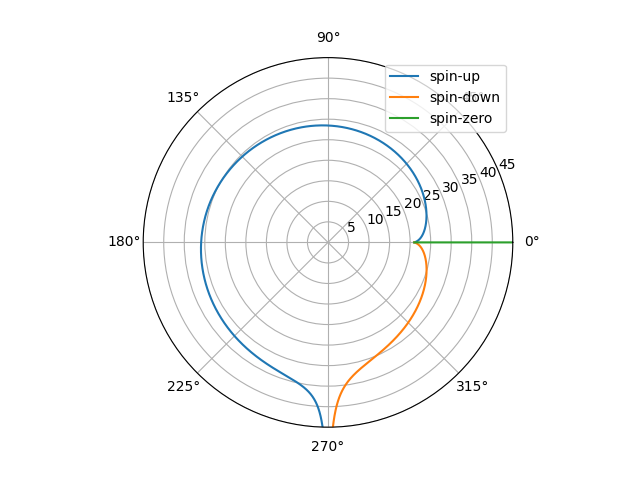
\includegraphics[width=\linewidth]{trajectory.png}
		\caption{The trajectories of a spin-up, spin-down and a spin-zero particle, $\hbar /m = 0.01$, $M=10$, $R=21$}
		\label{fig:trajectories}
	\end{figure}
	
	\subsection{Tangential geodesic}
	
	The geodesic equation can be reduced to,
	
	\begin{equation}
		H = \frac{1}{2} \left(\frac{d r}{d \tau}\right)^2 + V_{eff}(r) = const
	\end{equation} 
	
	

	
	
	
	
	
	
	
	
	
	
	
	
	
	
	
	
	
	
	
	
	
	
	
	

	

	
	
	
	
	%%\printbibliography
	
	
\end{document}

